\title{Aula 6 - Cifras de Fluxo}

\author{Prof. Gabriel Rodrigues Caldas de Aquino}

\institute
{
    Instituto de Computação \\
    Universidade Federal do Rio de Janeiro\\
    gabrielaquino@ic.ufrj.br% Your institution for the title page
}
\date{Compilado em: \\ \today} % Date, can be changed to a custom date

%----------------------------------------------------------------------------------------
%    PRESENTATION SLIDES
%----------------------------------------------------------------------------------------



\begin{frame}
    % Print the title page as the first slide
    \titlepage
\end{frame}

\begin{frame}{Princípio de Kerckhoffs}
    \begin{block}{Definição}
        O Princípio de Kerckhoffs, formulado por Auguste Kerckhoffs no século XIX, afirma que a segurança dos dados encriptados deve depender apenas da chave usada, mesmo que o método ou algoritmo seja de conhecimento público.
    \end{block}

    \begin{block}{Implicação}
        Esse princípio denuncia a falácia da \textit{segurança pela obscuridade}, evidenciando que, se a segurança depende do segredo do método, então o método é falho.
    \end{block}
\end{frame}



\begin{frame}{Cifras de fluxo}
    \begin{itemize}
        \item Uma \textbf{técnica de substituição} é aquela em que as letras do texto claro são substituídas por outras letras, números ou símbolos.  Se o texto claro for visto como uma sequência de bits, então a substituição envolve trocar
              padrões de bits de texto claro por padrões de bits de texto cifrado.
    \end{itemize}

    \begin{itemize}
        \item \textbf{Cifra de fluxo}: Encripta um fluxo de dados digital um bit ou um byte por vez.
        \item Exemplos clássicos:
              \begin{itemize}
                  \item Vigenère autochaveada
                  \item Vernam
              \end{itemize}
    \end{itemize}
\end{frame}

\begin{frame}{Da aula passada: Cifra de Fluxo: Vernam (One-Time Pad)}

    \begin{itemize}
        \item Cada bit do texto claro é combinado com um bit da chave usando \textbf{XOR}.
        \item Se a chave for tão longa quanto a mensagem e aleatória, temos o \textbf{One-Time Pad}, inquebrável.

              \begin{itemize}
                  \item É uma versão ideal da cifra de Vernam.
                  \item O fluxo de chaves ($k_i$) tem o mesmo tamanho do fluxo de bits do texto claro ($p_i$).
                  \item Se a chave for realmente aleatória, a cifra é \textbf{inquebrável}.
                  \item Limitação: o fluxo de chaves precisa ser \textbf{pré-distribuído} de forma segura.
                  \item Problema prático: inviável para grandes volumes de tráfego devido à logística de distribuição.
              \end{itemize}


        \item Se a chave for curta e repetida, a segurança é comprometida.
    \end{itemize}




\end{frame}



\begin{frame}{XOR: Base das Cifras de Fluxo}
    \begin{columns}
        \column{0.45\textwidth}
        \centering
        \textbf{Tabela-verdade da função XOR}
        \vspace{0.3cm}

        \begin{tabular}{|c|c|c|}
            \hline
            A & B & S \\
            \hline
            0 & 0 & 0 \\
            0 & 1 & 1 \\
            1 & 0 & 1 \\
            1 & 1 & 0 \\
            \hline
        \end{tabular}

        \vspace{0.2cm}
        \scriptsize{Onde $S = A \oplus B$}

        \column{0.55\textwidth}
        %

        \textbf{Exemplo de Encriptação e Decriptação}\\
        Para cifrar (c) = $TEXTO \oplus CHAVE$:
        \begin{tabular}{|c|c|}
            \hline
            Texto claro (p) & 1 \; 0 \; 1 \; 1 \\
            \hline
            Chave (k)       & 0 \; 1 \; 0 \; 1 \\
            \hline
            Cifrado (c)     & 1 \; 1 \; 1 \; 0 \\

            \hline
        \end{tabular}



        Para decriptar (d): $CIFRADO \oplus CHAVE$: \\[0.2cm]

        \begin{tabular}{|c|c|}
            \hline
            Cifrado (c)     & 1 \; 1 \; 1 \; 0 \\
            \hline
            Chave (k)       & 0 \; 1 \; 0 \; 1 \\
            \hline
            Texto claro (p) & 1 \; 0 \; 1 \; 1 \\
            \hline
        \end{tabular}
        %
    \end{columns}
\end{frame}

\begin{frame}{Cifra de fluxo}



    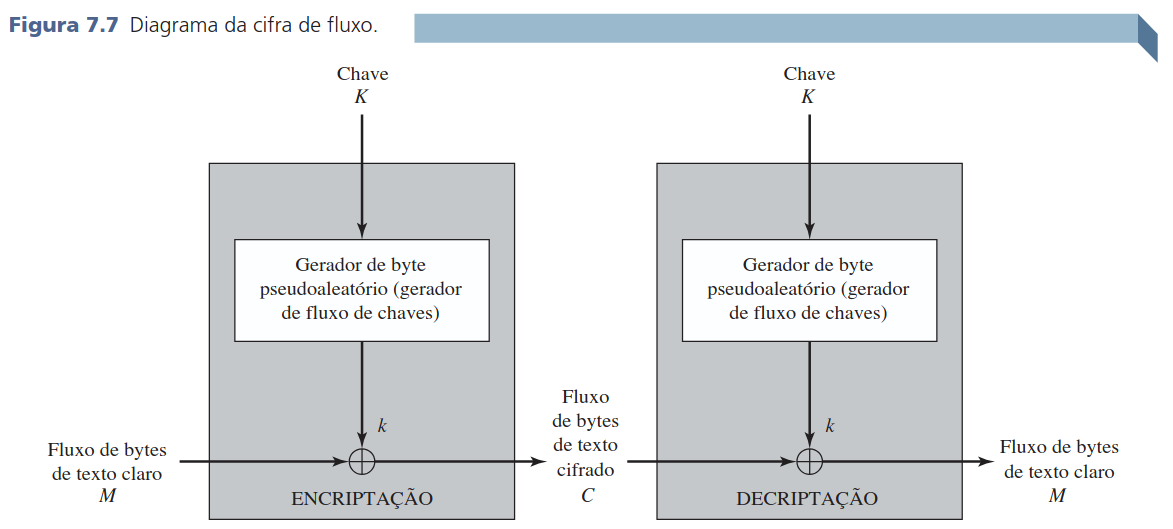
\includegraphics[width=\linewidth]{Figuras/Cifra-de-fluxo.png}



\end{frame}


\begin{frame}{Cifra de Fluxo}
    \begin{itemize}

        \item Uma cifra de fluxo típica encripta um byte de texto claro por vez, embora possa operar sobre um bit ou unidades maiores.
        \item Uma chave é inserida em um gerador de bits pseudoaleatórios que produz um fluxo de números de 8 bits aparentemente aleatórios.
        \item A saída do gerador, chamada \textit{fluxo de chaves}, é combinada byte a byte com o texto claro usando a operação \textbf{OU exclusivo (XOR)} bit a bit.

    \end{itemize}
\end{frame}

\begin{frame}{Cifra de fluxo}



    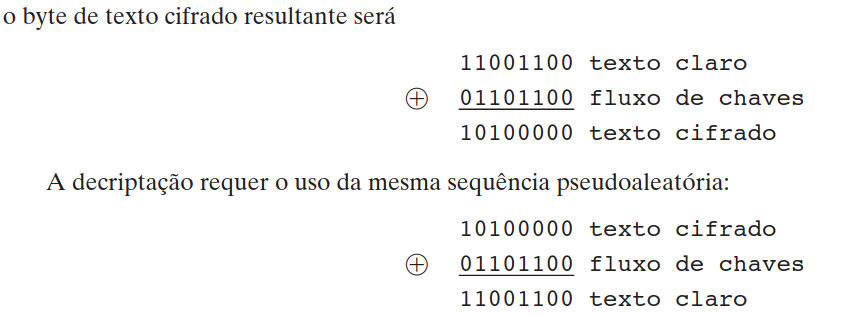
\includegraphics[width=\linewidth]{Figuras/xor-cifrado-fluxo.png}



\end{frame}


\begin{frame}{Geradores de Fluxo em Cifras de Fluxo}
    \begin{itemize}
        \item Por motivos práticos, o fluxo de bits é gerado por um \textbf{algoritmo} controlado por chave.
        \item O gerador deve produzir um fluxo \textbf{criptograficamente forte}.
              \begin{itemize}
                  \item Não deve ser possível prever partes futuras do fluxo a partir de partes já conhecidas.
              \end{itemize}
        \item Os usuários compartilham apenas a \textbf{chave de geração}.
        \item Cada usuário pode então produzir localmente o mesmo fluxo de chaves.
    \end{itemize}
\end{frame}

\begin{frame}{Cifras de Fluxo}
    \textbf{Semelhança com One-Time Pad:}
    \begin{itemize}
        \item Uma cifra de fluxo também encripta um fluxo de bits de texto claro com um fluxo de chave.
        \item No one-time pad, o fluxo de chave é \textbf{verdadeiramente aleatório}.
        \item Na cifra de fluxo, o fluxo de chave é \textbf{pseudoaleatório}, gerado por um algoritmo.
    \end{itemize}

    \textbf{Considerações de projeto para cifras de fluxo:}
    \begin{enumerate}
        \item A sequência de encriptação deverá ter um período grande?
        \item O fluxo de chaves deverá se aproximar o máximo possível das propriedades de um fluxo de número
              aleatório verdadeiro?
        \item A  chave precisa ser suficientemente longa?
    \end{enumerate}
\end{frame}

\begin{frame}{Período de Repetição em Cifras de Fluxo}
    \textbf{Sequência de Encriptação:}
    \begin{itemize}
        \item A sequência de bits gerada pelo gerador pseudoaleatório deve ter \textbf{um período longo}.
        \item O gerador produz um fluxo determinístico de bits que eventualmente se repete.
        \item Quanto maior o período, mais difícil é a criptoanálise.
    \end{itemize}

    \textbf{Relação com a cifra de Vigenère:}
    \begin{itemize}
        \item Na Vigenère, uma palavra-chave curta se repete, facilitando ataques por análise de frequência.
        \item Na cifra de fluxo, um período maior no gerador pseudoaleatório reduz padrões repetitivos, aumentando a segurança.
    \end{itemize}
\end{frame}

\begin{frame}{Propriedades de Aleatoriedade do Fluxo de Chaves}
    \textbf{Requisitos para o fluxo de chaves em cifras de fluxo:}
    \begin{itemize}
        \item O fluxo deve se aproximar de \textbf{um número aleatório verdadeiro}.
        \item Deve conter aproximadamente o mesmo número de 1s e 0s.
        \item Se o fluxo for tratado como bytes, os 256 valores possíveis devem aparecer com frequência aproximadamente igual.
    \end{itemize}

    \textbf{Impacto na segurança:}
    \begin{itemize}
        \item Quanto mais aleatório o fluxo de chaves, mais aleatório será o texto cifrado.
        \item Isso dificulta a criptoanálise, pois padrões previsíveis são minimizados.
    \end{itemize}
\end{frame}

\begin{frame}{Tamanho da Chave em Cifras de Fluxo}
    \textbf{Considerações sobre a chave:}
    \begin{itemize}
        \item A saída do gerador de número pseudoaleatório depende da \textbf{chave de entrada}.
        \item Para proteção contra ataques de força bruta, a \textbf{chave deve ser suficientemente longa}.
        \item Assim como em cifras de bloco, recomenda-se \textbf{chaves de pelo menos 128 bits} com a tecnologia atual.
    \end{itemize}

    \textbf{Importância:} Uma chave curta compromete a segurança, mesmo que o gerador de fluxo seja forte.
\end{frame}

\begin{frame}{Comparação entre Cifras de Fluxo e de Bloco}
    \textbf{Segurança:}
    \begin{itemize}
        \item Uma cifra de fluxo bem projetada pode ser tão segura quanto uma cifra de bloco com a mesma \textbf{tamanho de chave}.
    \end{itemize}

    \textbf{Vantagens das cifras de fluxo:}
    \begin{itemize}
        \item Geralmente mais rápidas que cifras de bloco.
        \item Requerem menos código para implementação.
        \item Exemplo: RC4 pode ser implementado em poucas linhas.
    \end{itemize}
\end{frame}

\begin{frame}{Comparação entre Cifras de Fluxo e de Bloco}


    \textbf{Atenção:}
    \begin{itemize}
        \item Nos últimos anos, essa vantagem diminuiu com a introdução do AES, que é bastante eficiente em software.
        \item Técnicas de aceleração de hardware, como o AES Instruction Set da Intel, permitem executar uma rodada de encriptação/decriptação e geração de chave com grande velocidade.
        \item Ganhos de velocidade podem ser de cerca de uma ordem de grandeza em relação a implementações puramente em software.
    \end{itemize}
\end{frame}


\begin{frame}{Vantagens e Riscos das Cifras de Bloco e Fluxo}
    \textbf{Cifras de Bloco:}
    \begin{itemize}
        \item Permitem \textbf{reutilização de chaves} sem comprometer a segurança.
    \end{itemize}

    \textbf{Cifras de Fluxo:}
    \begin{itemize}
        \item Se dois textos claros forem encriptados com a mesma chave, a criptoanálise torna-se trivial.
        \item O XOR dos dois textos cifrados produz o XOR dos textos claros originais.
        \item Vulnerável especialmente quando os textos claros possuem padrões conhecidos, como strings de texto, números de cartão de crédito ou outros fluxos de bytes estruturados.
    \end{itemize}
\end{frame}

\begin{frame}{Escolha de Cifras: Fluxo vs. Bloco}
    \textbf{Cifras de Fluxo:}
    \begin{itemize}
        \item Adequadas para \textbf{encriptação/decriptação contínua} de dados.
        \item Ex.: canais de comunicação de dados, links de navegador/Web.
    \end{itemize}

    \textbf{Cifras de Bloco:}
    \begin{itemize}
        \item Indicadas para \textbf{blocos de dados} inteiros.
        \item Ex.: transferência de arquivos, e-mails, bancos de dados.
    \end{itemize}

    \textbf{Observação:} Ambos os tipos podem ser usados em praticamente qualquer aplicação, dependendo do projeto.
\end{frame}

\begin{frame}{Cifra de Fluxo RC4}
    \textbf{Descrição:}
    \begin{itemize}
        \item Criada em 1987 por Ron Rivest para a RSA Security.
        \item Tamanho de chave \textbf{variável}, operações orientadas a \textbf{byte}.
        \item Baseada em uma \textbf{permutação aleatória}.
    \end{itemize}

    \textbf{Características:}
    \begin{itemize}
        \item Período provavelmente maior que $10^{100}$.
        \item De 8 a 16 operações de máquina por byte de saída.
        \item Executa rapidamente em software.
    \end{itemize}

    \textbf{Hoje é considerado inseguro, mas ja teve uso:}
    \begin{itemize}
        \item SSL/TLS (comunicação navegador-servidor Web)
        \item WEP e WPA (padrão IEEE 802.11 LAN sem fio)
    \end{itemize}

    \textbf{Histórico:}
    \begin{itemize}
        \item Mantido como segredo comercial até 1994.
        \item Postado na Internet na lista Cypherpunks em setembro de 1994.
    \end{itemize}
\end{frame}

\begin{frame}{RC4: Inicialização e Operação}
    \textbf{Inicialização:}
    \begin{itemize}
        \item Chave de tamanho variável: 1 a 256 bytes (8 a 2048 bits).
        \item Vetor de estado $S$ de 256 bytes: $S[0], S[1], \dots, S[255]$.
        \item $S$ contém uma \textbf{permutação de todos os números de 0 a 255}.
    \end{itemize}

    \textbf{Operação (Encriptação/Decriptação):}
    \begin{itemize}
        \item Um byte $k$ é gerado a partir de $S$ selecionando uma entrada de forma sistemática.
        \item Cada vez que um byte $k$ é gerado, os elementos de $S$ são \textbf{novamente permutados}.
        \item A saída $k$ é usada para XOR com o byte do texto claro/cifrado:
              \[
                  c_i = p_i \oplus k, \quad p_i = c_i \oplus k
              \]
    \end{itemize}

    \begin{itemize}
        \item $p_i$
              i-ésimo  bit (ou byte)  do texto claro.

        \item $k$ byte (ou bit) gerado pelo gerador de fluxo da cifra RC4.

        \item  $c_i$
              i-ésimo byte (ou bit) do texto cifrado,
    \end{itemize}

\end{frame}

\begin{frame}{Inicialização do Vetor S no RC4}
    \begin{itemize}
        \item Defina o vetor de estado $S$ com 256 elementos:
              \[
                  S[0] = 0, \; S[1] = 1, \; \dots, \; S[255] = 255
              \]
        \item Crie um vetor temporário $T$ do mesmo tamanho que $S$.
        \item Preencha $T$ usando a chave $K$ de tamanho \texttt{keylen}:
              \begin{itemize}
                  \item Se \texttt{keylen} = 256, copie $K$ diretamente para $T$.
                  \item Caso contrário, copie os primeiros \texttt{keylen} bytes de $K$ para $T$, repetindo a chave tantas vezes quanto necessário até completar 256 elementos.
              \end{itemize}
    \end{itemize}
\end{frame}


\begin{frame}{RC4 - inicializacao}



    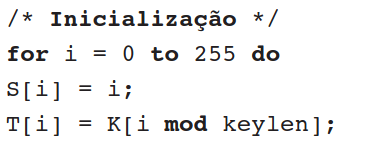
\includegraphics[width=\linewidth]{Figuras/rc4-inicializacao.png}



\end{frame}

\begin{frame}{Exemplo - Inicialização do RC4 - Passo 1: Vetores S e T}
    \textbf{Chave:} \texttt{11111001 (1 byte)}

    \bigskip

    \textbf{Vetor S:} Inicialmente com 256 elementos em ordem crescente:
    \[
        S = [0, 1, 2, 3, \dots, 255]
    \]

    \textbf{Vetor T:} Criado a partir da chave, repetida até ter 256 elementos:
    \[
        T = [11111001, 11111001, 11111001, \dots] \text{(256 elementos)}
    \]

    \bigskip
    \textbf{Resumo:}
    \begin{itemize}
        \item S contém todos os números de 0 a 255.
        \item T é preenchido sequencialmente com os bytes da chave, repetindo-a se necessário.
    \end{itemize}
\end{frame}

\begin{frame}{RC4 - permutação}
    \begin{itemize}


        \item    Em seguida, usamos T para produzir a permutação inicial de S.
        \item Isso envolve começar com S[0] e ir até
              S[255], e, para cada S[i], trocar S[i] por outro byte em S, de acordo com um esquema ditado por T[i]
        \item Como a única operação sobre S é uma troca, o único efeito é uma permutação. S, ainda, contém todos os
              números de 0 a 255.

    \end{itemize}

    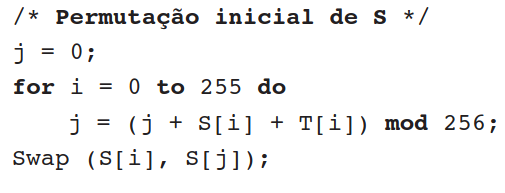
\includegraphics[width=\linewidth]{Figuras/rc4-permutacao-inicial.png}



\end{frame}

\begin{frame}{RC4 - geração do fluxo}
    \begin{itemize}


        \item    Uma vez que o vetor S é inicializado, a chave de entrada não é mais usada.
        \item A geração de fluxo é percorrer todos os elementos de S[i] e, para cada S[i], trocar S[i] por outro byte em S de acordo com um esquema
              ditado pela configuração atual de S.

        \item Depois que S[255] é atingido, o processo continua, começando novamente
              em S[0]:

    \end{itemize}

    \centering
    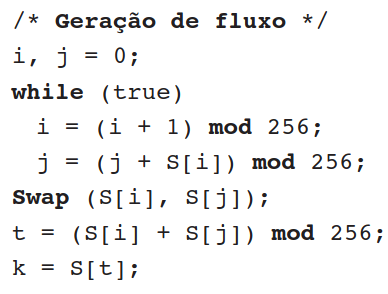
\includegraphics[width=0.4\linewidth]{Figuras/rc4-geracao-de-fluxo.png}

    \begin{itemize}
        \item Para encriptar, faça o XOR do valor k com o próximo byte do texto claro. Para decriptar, faça o XOR do
              valor k com o próximo byte do texto cifrado.
    \end{itemize}

\end{frame}


\begin{frame}{RC4 - big picture}


    \centering
    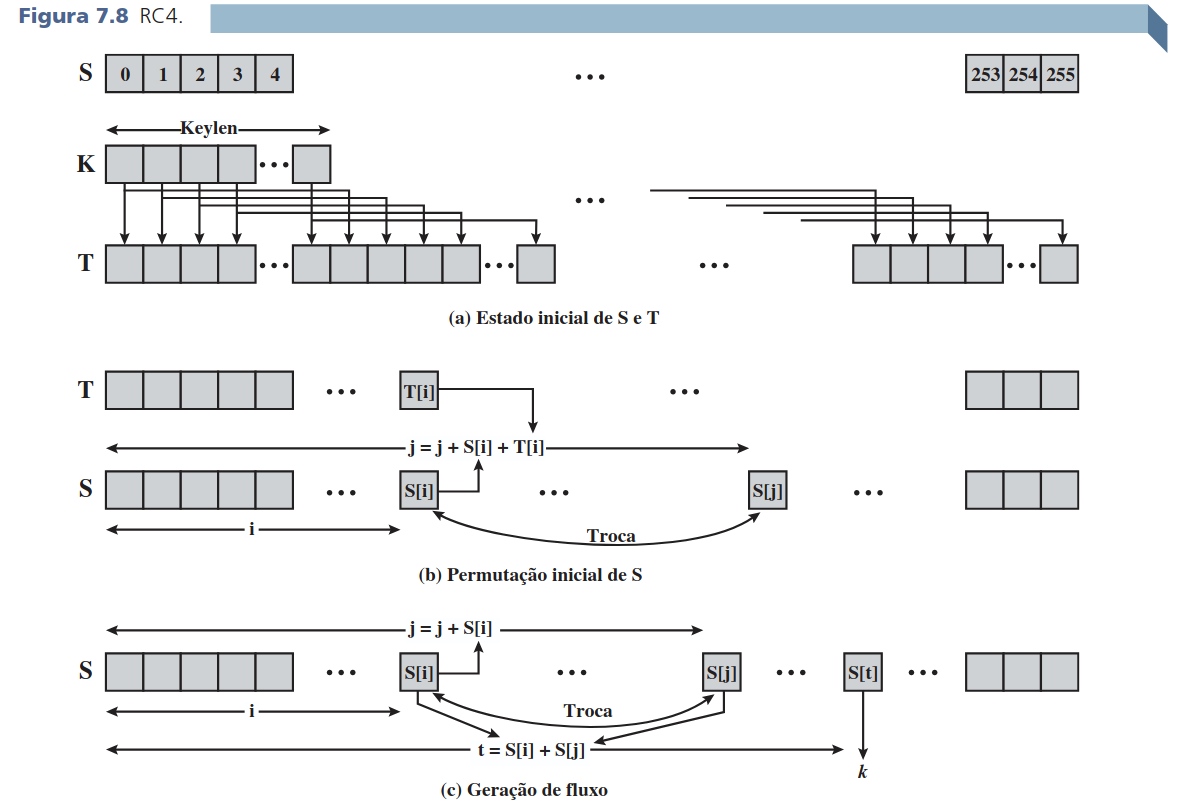
\includegraphics[width=0.75\linewidth]{Figuras/rc4-big-picture.png}



\end{frame}


\begin{frame}{Força do RC4 e Vulnerabilidade no WEP}
    \textbf{Segurança do RC4:}
    \begin{itemize}
        \item RC4 é resistente a ataques práticos se a chave for suficientemente longa (ex: 128 bits).
        \item Muitos estudos analisaram métodos de ataque, mas não são práticos para chaves de tamanho adequado.
    \end{itemize}

    \textbf{Problema no WEP:}
    \begin{itemize}
        \item O protocolo WEP (para redes 802.11) mostrou-se vulnerável devido à forma de geração de chaves.
        \item O problema não está no RC4 em si, mas no uso incorreto da chave.
        \item O uso do WEP é desencorajado hoje em dia
    \end{itemize}


\end{frame}
